% Forecasting Average Traffic Speed on PEMS08 — Beamer deck
% Compile: pdflatex slides.tex   (theme Madrid; figures from reports/figures/)
\documentclass[aspectratio=169]{beamer}
\usetheme{Madrid}
\usecolortheme{whale}
\usepackage{booktabs}
\usepackage{amsmath}
\usepackage{graphicx}
\graphicspath{{../reports/figures/}}
\setbeamertemplate{navigation symbols}{}
\setbeamertemplate{caption}{\raggedright\insertcaption\par}
\setbeamerfont{frametitle}{size=\large}

\title[Traffic Speed Forecasting on PEMS08]{Forecasting Average Traffic Speed\\on the PEMS08 Sensor Network}
\subtitle{Single-horizon vs.\ multi-horizon graph neural networks}
\author{Vita Nagli\v{c} \and Matev\v{z} Rom \and Nace Kova\v{c}i\v{c}}
\institute{Artificial Intelligence}
\date{}

\begin{document}

\begin{frame}
  \titlepage
\end{frame}

\begin{frame}{Outline}
  \tableofcontents
\end{frame}

% ============================================================================
\section{Introduction}
% ============================================================================
\begin{frame}{Introduction}
  \begin{itemize}
    \item A road network is covered by traffic sensors that measure speed every 5 minutes.
    \item \textbf{Goal:} given the recent past, forecast the average speed (mph) at each sensor for the near future.
    \item Why it matters: travel-time estimation, routing, congestion warnings, traffic management.
    \item It is a regression problem on a spatio-temporal graph:
    \begin{itemize}
      \item \textbf{nodes} = sensors, \textbf{edges} = road connections,
      \item each node carries a \textbf{time series} (speed, flow, occupancy).
    \end{itemize}
    \item We build two neural networks:
    \begin{itemize}
      \item \textbf{NN1} --- predict speed exactly 60 minutes ahead;
      \item \textbf{NN2} --- predict the whole curve from +5 to +60 minutes.
    \end{itemize}
  \end{itemize}
\end{frame}

% ============================================================================
\section{Dataset}
% ============================================================================
\begin{frame}{The PEMS dataset --- focus on PEMS08}
  \begin{columns}[T]
    \begin{column}{0.54\textwidth}
      \begin{itemize}
        \item \textbf{PeMS} = California ``Performance Measurement System'': loop detectors on freeways (PEMS03/04/07/08 are standard forecasting benchmarks).
        \item \textbf{PEMS08} (this work): district 8, Jul--Aug 2016.
      \end{itemize}
      \vspace{0.4em}
      \footnotesize
      \begin{tabular}{ll}
        \toprule
        Property & Value \\
        \midrule
        Sensors (nodes) & 170 \\
        Time steps & 17\,856 \\
        Resolution & 5 minutes \\
        Duration & $\sim$2 months \\
        Channels & flow, occupancy, speed \\
        Graph & directed, distance-weighted \\
        \bottomrule
      \end{tabular}
    \end{column}
    \begin{column}{0.46\textwidth}
      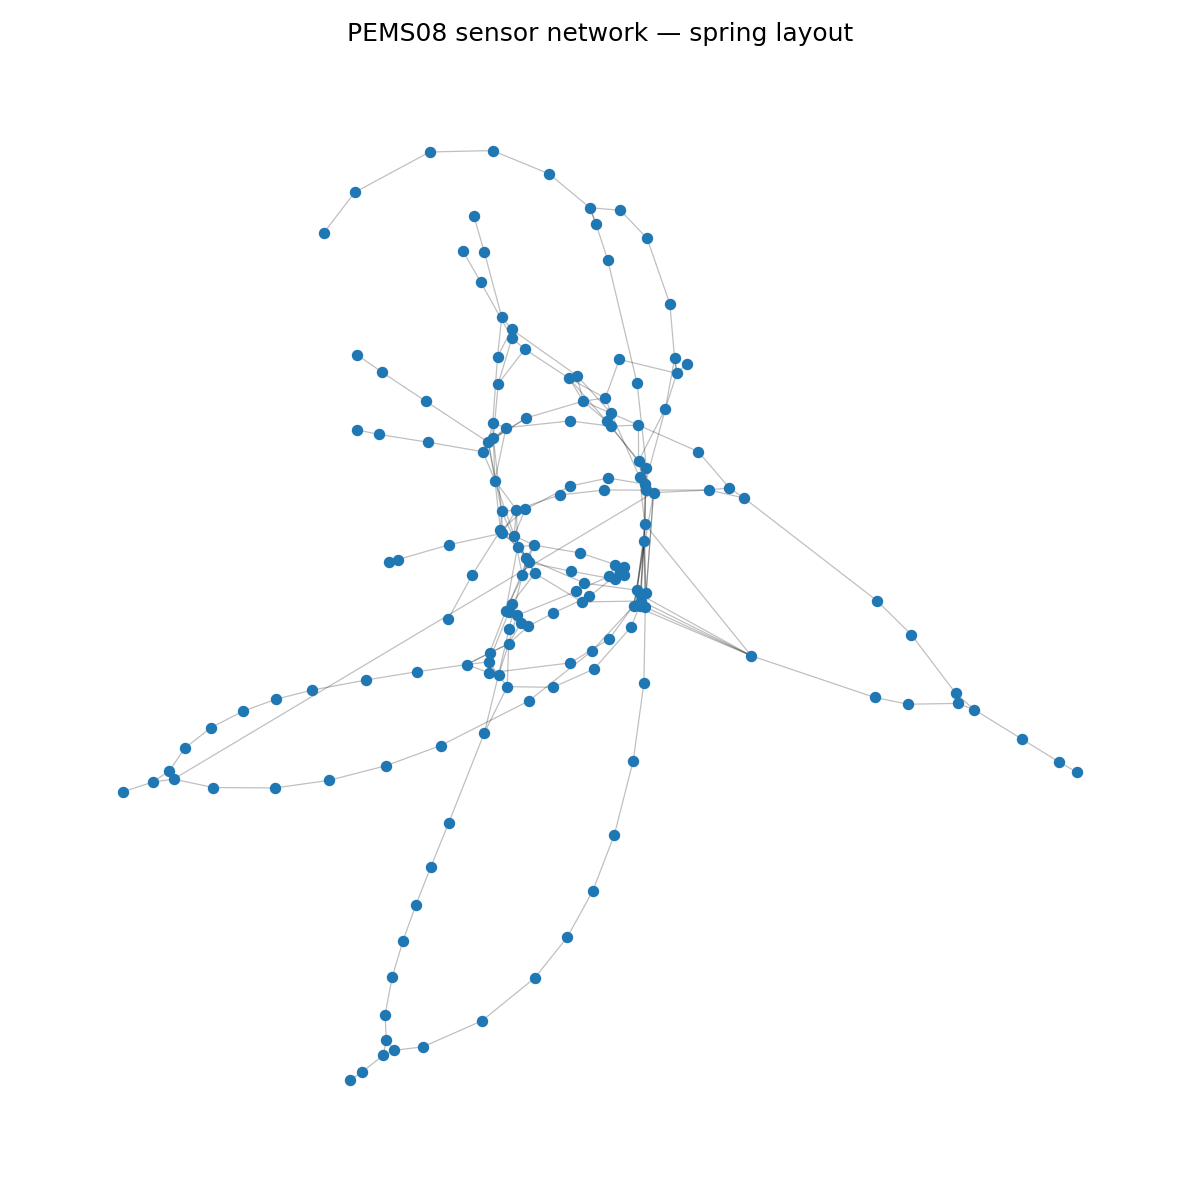
\includegraphics[width=\linewidth]{pems08_network_layout.png}
    \end{column}
  \end{columns}
\end{frame}

\begin{frame}{The sensor graph --- network structure}
  \begin{columns}[c]
    \begin{column}{0.5\textwidth}
      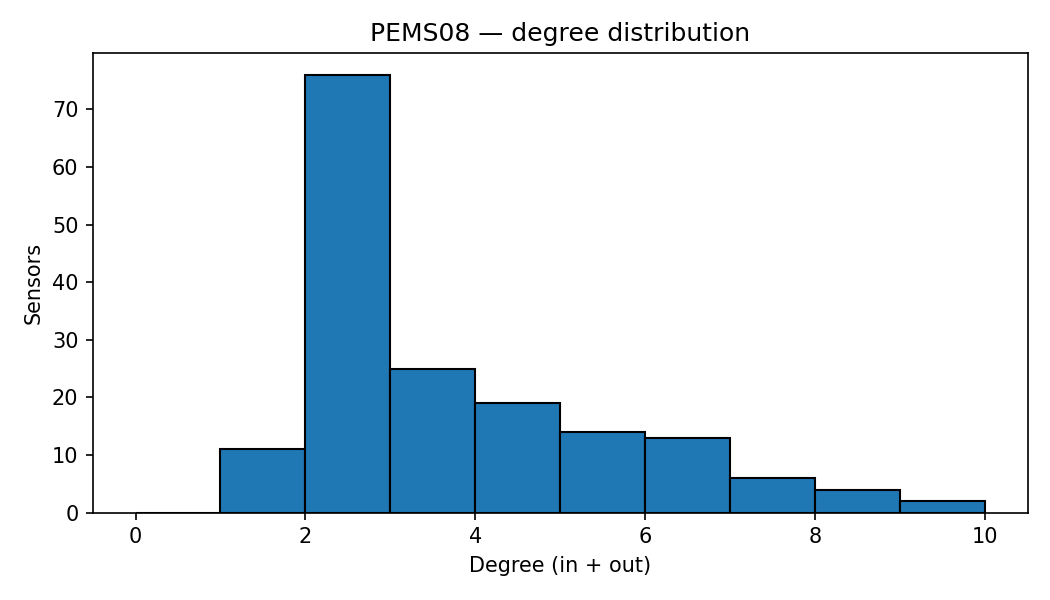
\includegraphics[width=\linewidth]{pems08_degree_distribution.png}
    \end{column}
    \begin{column}{0.5\textwidth}
      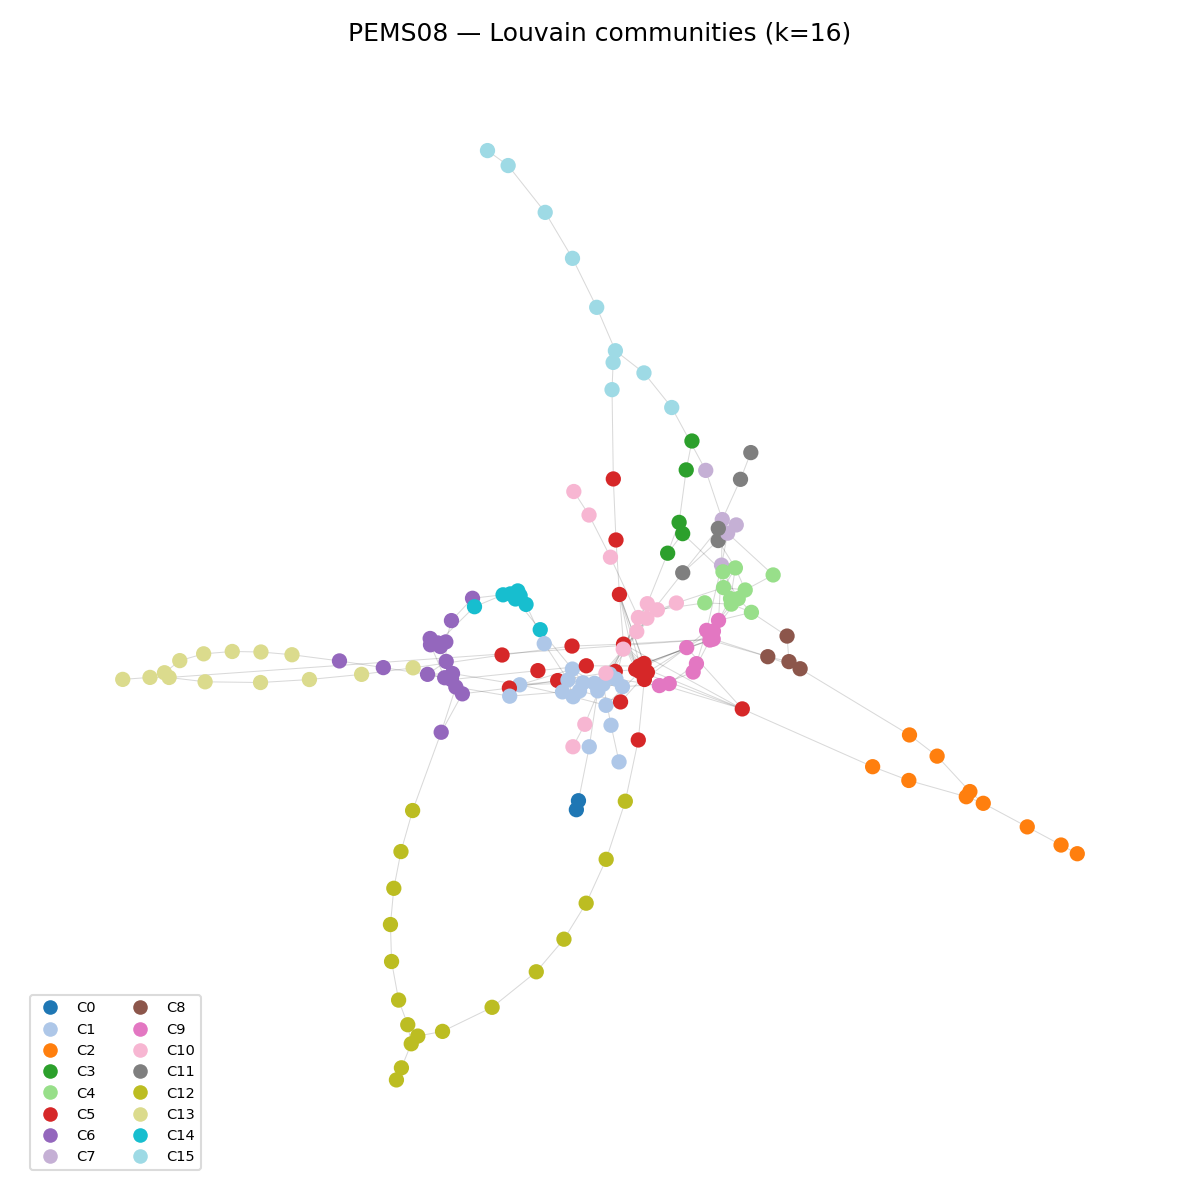
\includegraphics[width=\linewidth]{pems08_communities.png}
    \end{column}
  \end{columns}
  \begin{itemize}
    \item Low, bounded degree: most sensors have only 2--3 neighbours (max $\sim$10 at interchanges), with no high-degree hubs --- the signature of a road network (unlike scale-free social / web graphs).
    \item Louvain finds $\sim$16 communities that trace highway corridors / sub-routes.
    \item $\Rightarrow$ speeds propagate locally along roads --- this is what a graph model exploits.
  \end{itemize}
\end{frame}

\begin{frame}{Channels \& daily congestion}
  \begin{columns}[T]
    \begin{column}{0.57\textwidth}
      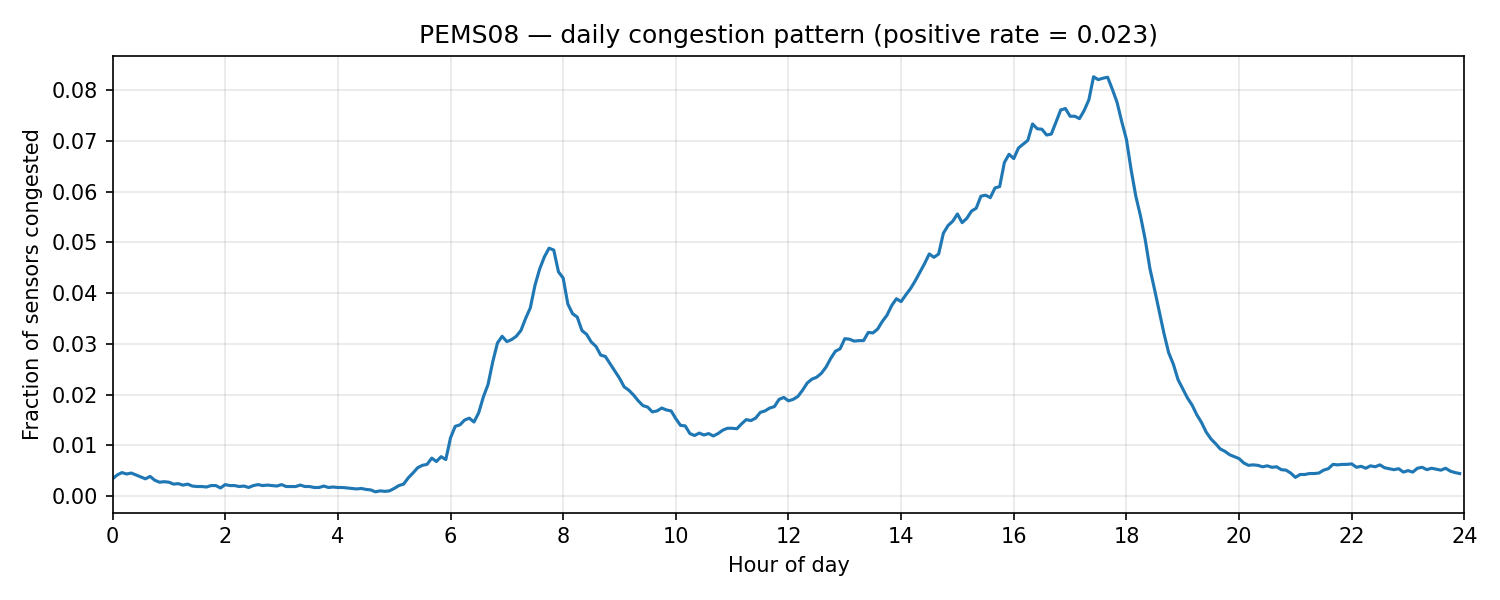
\includegraphics[width=\linewidth]{pems08_daily_congestion.png}
      \vspace{0.3em}
      \footnotesize\centering
      Fraction of sensors congested vs hour of day.
    \end{column}
    \begin{column}{0.43\textwidth}
      \footnotesize
      \begin{itemize}
        \item Each sensor logs \textbf{flow}, \textbf{occupancy}, \textbf{speed} every 5 min --- we forecast speed.
        \item Congestion $=$ speed $<$ 60\% of a sensor's free-flow (95th-percentile) speed: per-sensor \& relative, not a fixed mph cutoff.
        \item Rare overall ($\sim$2.3\%) but concentrated in AM ($\sim$8\,h) and PM ($\sim$17\,h) rush peaks; near zero overnight.
        \item Strong daily periodicity $\Rightarrow$ time-of-day features; congestion is the rare hard case.
      \end{itemize}
    \end{column}
  \end{columns}
\end{frame}

% ============================================================================
\section{Neural Network 1: 60 minutes ahead}
% ============================================================================
\begin{frame}{NN1 --- what goes in and what comes out}
  \textbf{Task:} for each sensor, predict its speed \textbf{one hour from now}.
  \begin{itemize}
    \item \textbf{Input (what the model sees):} the \textbf{last hour} of data from every sensor
          --- 12 readings, one every 5 minutes.
    \item \textbf{Output (what it predicts):} one number per sensor --- the speed in \textbf{60 minutes}.
    \item \textbf{Each reading gives 10 numbers per sensor:}
    \begin{itemize}
      \item the 3 measured signals: flow, occupancy, speed;
      \item the time of day and day of week (so it learns rush-hour patterns);
      \item the average of its road-neighbours' signals (what nearby traffic is doing).
    \end{itemize}
    \item We do \textbf{not} add ``speed X minutes ago'' features --- the last hour is already in the input.
  \end{itemize}
\end{frame}

\begin{frame}{NN1 --- split, normalisation, no leakage}
  \begin{itemize}
    \item Temporal (chronological) split: 60\% train / 20\% val / 20\% test.
    \begin{itemize}
      \item train = past, test = future $\Rightarrow$ mimics real deployment.
      \item not random k-fold: autocorrelation would leak the future and inflate scores.
    \end{itemize}
    \item Per-sensor z-score normalisation using \textbf{training statistics only}
    (features and target); predictions denormalised back to mph for all metrics.
    \item No look-ahead: a gap of W = 12 steps is dropped at each split boundary, so an input window never crosses into another split.
  \end{itemize}
\end{frame}

\begin{frame}{NN1 --- architecture (GCN-GRU) \& training}
  \textbf{Spatial (per time step) --- graph convolution:}
  \[ H = \mathrm{ReLU}(A\,X\,W_{gcn}),\quad
     A = \alpha\,A_{\text{fixed}} + (1-\alpha)\,\tilde A,\quad
     \tilde A = \mathrm{softmax}(\mathrm{ReLU}(E_1 E_2^{\top})) \]
  \begin{itemize}
    \item Adaptive adjacency $\tilde A$: a learned graph (captures correlations geometry misses).
    \item Residual $H = \mathrm{GCN}(X) + \mathrm{Linear}(X)$: keeps each sensor's own signal.
    \item \textbf{Temporal:} 2-layer GRU over the 12 steps (shared across sensors).
    \item \textbf{Head:} $\mathrm{Linear}(\text{hidden}\to 1)$ $\Rightarrow$ one speed (60 min). No sigmoid.
    \item \textbf{Training:} Huber loss ($\delta=1$), Adam (lr $10^{-3}$), early stopping on val MAE,
          seed 42, $\sim$56k params, trained on Apple-Silicon GPU (MPS).
  \end{itemize}
\end{frame}

% ============================================================================
\section{Neural Network 2: interval [+5, +60] minutes}
% ============================================================================
\begin{frame}{NN2 --- predicting the whole interval [+5, +60] min}
  \textbf{Task:} for every sensor, predict speed at all 12 steps 5, 10, \dots, 60 min ahead.
  \begin{itemize}
    \item ``Any segment at any near-future time'' --- the data lives on a 5-min grid.
    \item \textbf{Target} grows from [170] to [170, 12] (one value per horizon).
    \item Same 10 features, same 12-step input window as NN1.
    \item Standard benchmark setup (DCRNN, Graph WaveNet report 15/30/60 min jointly).
  \end{itemize}
  \vspace{0.3em}
  Both models are kept in the code (flag \texttt{-{}-single-horizon} selects NN1);
  NN2 is the default. Neither overwrites the other.
\end{frame}

\begin{frame}{NN2 --- what changes vs NN1}
  \begin{itemize}
    \item \textbf{Same} spatial GCN + adaptive adjacency + residual, \textbf{same} GRU, \textbf{same} split, normalisation, loss, training recipe.
    \item \textbf{Only the output head changes:}
    \[ \mathrm{Linear}(\text{hidden}\to 1)\ \Longrightarrow\ \mathrm{Linear}(\text{hidden}\to 12) \]
    \item Output shape per sample: $[N] \Rightarrow [N, 12]$; Huber loss summed over all 12 horizons.
    \item Predicting all horizons jointly acts as multi-task regularisation (one model, full curve).
    \item Cost: $\sim$60k params (vs $\sim$56k) --- essentially free.
  \end{itemize}
\end{frame}

% ============================================================================
\section{Results}
% ============================================================================
\begin{frame}{Results --- NN1 vs NN2 vs baselines}
  \centering
  \begin{table}
  \begin{tabular}{lccc}
    \toprule
    Model (test set) & MAE & RMSE & MAPE \\
    \midrule
    Persistence (avg over 5--60 min) & 1.6133 & 3.7811 & 3.08\% \\
    Persistence (60 min only)        & 2.1403 & 4.9692 & 4.21\% \\
    \midrule
    NN1 --- single-horizon (60 min) & 1.7979 & 4.4583 & 4.13\% \\
    NN2 --- multi-horizon (60 min)  & \textbf{1.7677} & 4.2927 & 3.98\% \\
    NN2 --- multi-horizon (avg)     & \textbf{1.4897} & 3.6037 & 3.23\% \\
    \bottomrule
  \end{tabular}
  \end{table}
  \begin{itemize}
    \item At 60 min, NN2 matches/beats NN1 while \emph{also} covering all shorter horizons.
    \item NN2 beats the average persistence by +7.7\% --- and that average is hard (see next slide).
  \end{itemize}
\end{frame}

\begin{frame}{Results --- the crossover (per-horizon MAE)}
  \begin{columns}[T]
    \begin{column}{0.62\textwidth}
      \includegraphics[width=\linewidth]{pems08_results_crossover.png}
    \end{column}
    \begin{column}{0.38\textwidth}
      \textbf{Key finding}
      \begin{itemize}
        \item Persistence is near-perfect short-term (speed barely changes in 5 min).
        \item The model overtakes at $\sim$20 min and the gap grows: +17.4\% at 60 min.
        \item $\Rightarrow$ judge models per horizon, not by a single average.
      \end{itemize}
    \end{column}
  \end{columns}
\end{frame}

\begin{frame}{Results --- ablation (each component helps)}
  \centering
  \includegraphics[width=0.7\linewidth]{pems08_results_ablation.png}
  \begin{itemize}
    \item Fixed-graph \textbf{base} is weakest; + adaptive adjacency and + residual each lower MAE.
    \item Same trend for NN1 and NN2 --- the gains come from architecture, not scale.
  \end{itemize}
\end{frame}

\begin{frame}{Conclusions}
  \begin{itemize}
    \item Two graph neural networks forecast PEMS08 speed: NN1 (60 min) and NN2 (full +5\dots+60 min curve).
    \item GCN + learned adjacency + residual + GRU beats strong baselines at the horizons that matter.
    \item NN2 gives the whole forecast curve from one model, matching NN1 at 60 min --- the more useful, practical choice.
    \item Crossover insight: short-term is owned by persistence; learned models win long-term.
    \item Future work: bidirectional diffusion, node-specific weights, temporal attention, congestion-weighted loss.
  \end{itemize}
\end{frame}

\end{document}
